% Section III: Data and Exploratory Analysis. Numbers:
%   results/metrics/eda_summary.json (scans, users, phones, groups, dates,
%     WAPs, readings, 0.77 m per data meter, new phones),
%   results/metrics/cleaning.csv (76 / 634 / 508 removed, 18,719 left).
% "Mostly from one phone": 430 of the 508 scans with a reading of -30 dBm or
% stronger come from phone 19 (count with indoorloc.data on trainingData.csv).
\section{Data and Exploratory Analysis}\label{sec:data}

\begin{figure}[t]
  \centering
  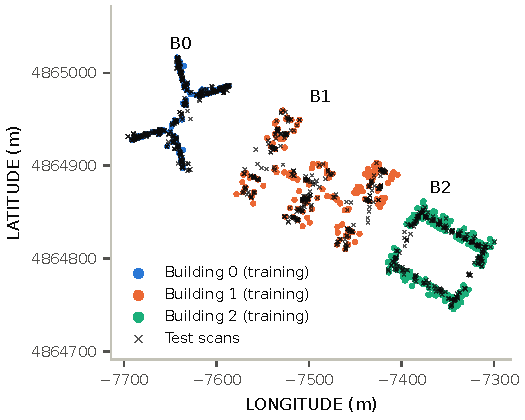
\includegraphics[width=0.9\columnwidth]{eda_campus_map.pdf}
  \caption{Where the scans were taken: training positions colored by building
  and test scans as crosses (Web-Mercator meters). Most test scans lie close
  to training positions.}
  \label{fig:campus}
\end{figure}

UJIIndoorLoc~\cite{torres2014ujiindoorloc} is dataset~310 of the UCI Machine
Learning Repository, recorded with smartphones in three buildings of
Universitat Jaume~I in Spain (Fig.~\ref{fig:campus}). Buildings~0 and~1 have
four floors and building~2 has five: 13 building--floor classes. Each row is
one scan: the RSSI of 520 WAPs, the building, floor and position, and the user
and phone ids. Positions are Web-Mercator meters; one such meter is about
0.77~m on the ground, and we report all errors in these dataset meters.

We train on the file \texttt{trainingData.csv}: 19,937 scans recorded from
30~May to 20~June 2013 by 18 users with 16 phones. Our \emph{test set} is the
UCI file \texttt{validationData.csv}: 1,111 scans recorded from 19~September to
8~October 2013 with 11 phones. It is hard for three reasons: it was recorded
about three months after the last training scan; 9 of its 11 phones never
appear in training, and they took 64.3\% of the test scans; and 55 of the WAPs
it hears are never heard in training, so no model can use them.

A scan hears only a few WAPs (17.82 on average in the cleaned training data,
16.48 in the test set), so 96.6\% of the training readings are ``not heard''.
The files store ``not heard'' as $+100$, which would look like the strongest
possible signal. We replace it by $-110$~dBm in both files: weaker than the
weakest real reading ($-104$~dBm), so ``not heard'' means ``very weak''.

We clean only the training file; the test file is used exactly as published.
In this order, we drop scans that hear no WAP (76), exact duplicate rows (634)
and scans with any reading of $-30$~dBm or stronger (508), which are
implausibly strong and come mostly from one phone. This leaves 18,719 training
scans. We keep only the 464 WAP columns heard in the cleaned training data,
because a WAP that is never heard tells a model nothing. Users who shared a
phone form one group, so the 18 training users form 16 user--device groups,
which we use for a fair split (Section~\ref{sec:method}).
